% Mini Paper
% CMSC 197 Machine Learning
% Hannah Bella C. Arceño and Jan Kristine A. Mosong
% January 2023
%
\documentclass[runningheads]{llncs}
% \documentclass[12pt, a4paper]{article}
%
\usepackage{graphicx}
\usepackage{indentfirst}

\begin{document}
%
\pagenumbering{roman}
\title{Contributing Factors to Twitch Viewership}
%
\author{Hannah Bella C. Arceño \and Jan Kristine A. Mosong \and Ara Abigail E. Ambita}
{\tt{hcarceno@up.edu.ph, jamosong@up.edu.ph}}
%
\authorrunning{Arceño, Mosong, Ambita}

% First names are abbreviated in the running head.
% If there are more than two authors, 'et al.' is used.
%

\institute{University of the Philippines Visayas, Miagao, Iloilo, Philippines
\email{ipo.upvisayas@up.edu.ph}\\
\url{https://www.upv.edu.ph}}
%
\maketitle
%
\begin{abstract}
    Streaming platforms provided career or earning opportunities for streamers. Twitch streamers with high stream views in particular, get discovered for brand advertisements and some are recruited for professional career. However, there are only few studies that explore the factors that affect streaming views. Understanding the fundamental factors that affect stream viewership is helpful for strategies in increasing stream views, which may be of help to aspiring streamers as well. This paper focused on finding the significant contributors to Twitch stream viewership. Five (5) models were built with Linear regression, using different combinations of features from the dataset. The best model earned an accuracy=0.829 or 82.9\%. Based on the model, the factors that contribute the most to the average number of viewers per stream are watch time, (total) stream time (in a year), number of peak viewers, number of followers, and whether partnered with Twitch and feature mature content. \\
   \keywords{Twitch  \and streaming \and views}
\end{abstract}
%
%
\pagenumbering{arabic}
\section{Introduction}
With the rising popularity of the gaming industry, streaming platforms such as Twitch began to rise which allowed gamers to share their content online with other game enthusiasts. Gaining more than two million concurrent viewers monthly \cite{twitchtracker}, the platform provides career-earning opportunities for its streamers through advertisement revenue. \\

Gaining high stream views is one of many ways to establish a career in Twitch. Streamers with high Twitch stream views have higher probabilities of earning more while streaming on the platform, such as Ninja, Shroud, and TimTheTatman. However, there have only been a few research on factors that affect Twitch views. \\

A study by Malm and Friberg explored the prediction of the average number of viewers of a sponsored stream using past available data. The study concluded that the past viewership numbers of a stream and other features such as the type of game and similar genres accurately predict the number of viewers of a recent stream \cite{malm2022viewership}.\\ 

Another study by L$\hat{e}$ et al. aimed to determine what factors play a part in the success of streamers. They discovered that the common factors among successful streamers were the duration of a stream, the number of streams per week, and the type of content. Live streams of successful streamers did not exceed five (5) hours and had a combination of gaming and non-gaming content posted at least five times a week \cite{le2021study}.  \\

% Additionally, the use of social media and marketing tactics to increase audience and build their online presence are essential components of content creation on any streaming platform. These plans of action could assist streamers who want to start their careers or use the platform as a source of revenue in concentrating their efforts on self-promotion, not just for the established streamers but also the up-and-coming ones. \\

Understanding the fundamental factors that affect stream viewership is advantageous for designing strategies to increasing stream views. This paper focused on finding the significant contributors to Twitch viewership. Particularly, the study aimed to explore whether the number of followers and total stream time correlates with viewership.

\section{Methodology}
This section delineates the implementation of the study. Actual implementation can be found in the Jupyter Notebook\footnote{Jupyter Notebook: https://github.com/yourstrulyhb/197-ML-mini-paper/blob/main/Contributing\%20Factors\%20to\%20Twitch\%20Viewership.ipynb}.

\subsection{Data Preparation}
\subsubsection{Dataset}
The dataset\footnote{Dataset found in https://www.kaggle.com/datasets/aayushmishra1512/twitchdata} was obtained from an online platform called Kaggle, a website that allows experts and learners of the data science and machine learning community to distribute their own dataset and use GPU-integrated notebooks such as Jupyter for others to view and work on \cite{uslu_2022}. \\

The downloaded dataset consisted of 1000 records that takes a look at the applicable data related to Twitch users namely: Channel, Watch time (minutes), Stream time (minutes), Peak viewers, Average viewers, Followers, Followers gained, Views gained, Partnered, Mature, and Language.\\
\\Channel - refers to the Twitch channel name.\\
Watch time (minutes) - refers to the total watch time in the past year\footnote{Past year pertains to the year 2019.} in minutes.\\
Stream time (minutes) -  refers to the total stream time in the past year in minutes.\\
Peak viewers - refers to the highest amount of viewers in all streams in the past year.\\
Average viewers - refers to the average number of viewers per stream in the past year.\\
Followers - refers to the total number of followers of the streamer (by the time of data collection).\\
Followers gained - refers to the total number of followers gained in the past year.\\
Views gained - refers to the total number of views gained in the past year.\\
Partnered - refers to whether the Twitch channel is partnered with Twitch or not.\\
Mature - refers to whether the Twitch channel contains adult or explicit content.\\
Language - refers to the language spoken by the Twitch channel.\\

The independent variable in this dataset is the Channel column while the ten remaining columns are the dependent variables. The feature of interest is 'Average viewers' while other variables are potential predictors except 'Channel'.

\subsubsection{Cleaning the dataset}
Highly variable and non-quantifiable features such as 'Channel' and 'Language' were removed from the experimentation to avoid issues with quantitative data. Quantifiable features however, such as 'Partnered' and 'Mature', which have two options only, were transformed to numerical equivalents. \\

The raw dataset contained no missing values. But several outliers were identified which can significantly affect the development of the models. To improve accuracy of each model, rows or observations with outlier value for any of the numerical columns or features were removed. This reduced the size of the dataset from 1000 observations to 613 observations. 


\subsubsection{Standardizing the dataset}
The dataset was further standardized for efficient computation. Values under initially numerical features - Watch time(Minutes), Stream time(minutes), Peak viewers, Average viewers, Followers, Followers gained, and Views gained - were standardized.  For non-numerical columns such as Partnered and Mature, values were maintained (i.e. 0 and 1). \\

After standardization, the dataset was divided into training and testing datasets.

\subsection{Experimental Setups}
To effectively determine the factors or features that predict the average number of viewers per stream, the study was divided into three different setups:

\subsubsection{Setup 1} All variables or features in the dataset were used in building the model.

\subsubsection{Setup 2} Only the hypothesized features, number of followers and total stream time in a year, are used in building the model.

\subsubsection{Setup 3} Employ feature selection with Pearson correlation to select the best features in building the model. This setup is further divided into three correlation thresholds=[0.3, 0.4, 0.5]. The upper limit of correlation thresholds were bounded to 0.5 as higher thresholds resulted to all features being included (which is similar to Setup 1). \\

All in all, five (5) models were generated in the study. 

\subsection{Linear Regression}
This study employed Linear Regression in building models for each experimental setup. Linear Regression is a supervised learning algorithm used in machine learning. It is one of the algorithms capable of predicting or visualizing the relationship between two (or more) different features or variables \cite{nelson_2021}. It takes the form:
\begin{equation}y=a_0+a_1x+\epsilon\end{equation}
where Y is a dependent variable or target variable, X is an independent variable or predictor variable, $a_0$ is the intercept of the line, $a_1$ is the coefficient of the linear regression and $\epsilon$ is a random error.  \\

Specifically, the study employed Multiple Linear Regression to predict the average number of views per stream, as several variables were used in prediction or building the models.


\subsection{Tools and Packages}
Data processing, model building, and other computational processes were done using Jupyter Notebook, an interactive computing platform on the web. In pre-processing the data, and creation and evaluation of the model, Python packages of NumPy, pandas, and scikit-learn were used. To visualize data, Python packages of Matplotlib and Seaborn were utilized.\\


\subsection{Evaluation Metrics}
The evaluation metrics used in the study were: $ R^2 $, Mean Absolute Error (MAE), Mean Squared Error (MSE), Accuracy (Regression Score), Cross-Validation Mean. \\

$ R^2 $ score or the coefficient of determination is used to evaluate the performance of a linear regression model. It refers to the amount of variation in the output predicted using predictor(s). An $ R^2 $ score value lies between 0 and 1, where a value closer to 1 means a better regression fit. \\

On the other hand, Mean Absolute Error (MAE) is an evaluation metric that takes the average of all absolute errors between actual and predicted values. And Mean Squared Error (MSE) is the average of the squares of the errors. The lower the value of MAE and MSE, the better the model fits the data.

\begin{equation}
    \textbf{MAE} = \sum_{i=1}^{D}|x_i-y_i|
\end{equation}

\begin{equation}
    \textbf{MSE} = \sum_{i=1}^{D}(x_i-y_i)^2
\end{equation}

Accuracy is described as the portion of correct predictions made among the total predictions. The values in this category lie between the values 0 and 1. A higher score shows that the model was able to properly determine the right prediction. \\

Cross-Validation Mean is a method used to determine whether the model generalizes itself to the test dataset. It partitions the dataset into sections of training and testing datasets then averages the final result to ensure model optimization. Cross-Validation Mean was used as secondary or verification metric to evaluate the models.


\section{Results and Discussion}

% ----- Model 1
\subsection{Model 1: Model with All Features}
Table \ref{tab:model1} show the intercept and coefficients of the model with all features: watch time (minutes), stream time (minutes), peak viewers, followers, followers gained, views gained, partnered and mature. \\

\begin{table}[h]
    \centering
    \caption{Model 1 intercept and coefficients from linear regression with all features.}
    \begingroup
    \setlength{\tabcolsep}{8pt} % Default value: 6pt
    \renewcommand{\arraystretch}{1.2} % Default value: 1
    
    \begin{tabular}{|p{.10\linewidth}|p{.12\linewidth}| p{.15\linewidth}|p{.15\linewidth}|p{.10\linewidth}|p{.14\linewidth}|}
        \hline
      & \textbf{Int} & \textbf{Watch time (minutes)} & \textbf{Stream time (minutes)} &	\textbf{Peak viewers}	& \textbf{Followers} \\
     \hline
     \textbf{Coef} & 0.2933015 & 0.726076 & -0.680808	& 0.05976	& 0.021213 \\
     \hline
     \end{tabular}
    
    \begin{tabular}{|p{.10\linewidth}|p{.12\linewidth}| p{.15\linewidth}|p{.15\linewidth}|p{.10\linewidth}|p{.14\linewidth}|}
        \hline
      & \textbf{Followers gained} & \textbf{Views gained} & \textbf{Partnered} & \textbf{Mature} &  \\
     \hline
     \textbf{Coef} & 0.018277	& 0.006903	& -0.312851	& 0.047701 & \\
    \hline
    \end{tabular}
    \label{tab:model1}
    \endgroup

\end{table}

Figure \ref{fig:model1} shows the scatterplot of the actual values against the predicted values of Model 1. The values closely fit the regression line, indicating that the model worked well in predicting the average number of viewers per stream. \\

\begin{figure}[h]
    \centering
    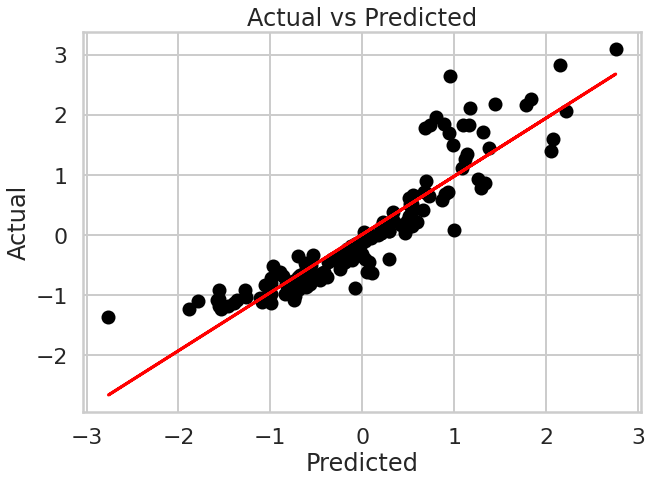
\includegraphics[width=0.6\linewidth]{figures/graphs/model_1_graph.png}
    \caption{Actual vs. Model 1 Predicted values }
  \label{fig:model1}
\end{figure}


% ----- Model 2
\subsection{Model 2: Model with Selected Features (Followers and Stream Time)}

Table \ref{tab:model2} shows the intercept and coefficients of the model with the hypothesized features, number of followers and total stream time in a year (minutes). \\

\begingroup
\setlength{\tabcolsep}{8pt} % Default value: 6pt
\renewcommand{\arraystretch}{1.2} % Default value: 1
\begin{table}[h]
    \centering
    \caption{Model 2 intercept and coefficients from linear regression with hypothesized features (Followers and Stream Time).}
    \begin{tabular}{|p{.10\linewidth}|p{.14\linewidth}|p{.20\linewidth}|p{.35\linewidth}|}
        \hline
      & \textbf{Int} & \textbf{Followers} & \textbf{Stream time (minutes)} \\
     \hline
     \textbf{Coef} & -0.014194 & 0.292029 & -0.491101	\\
     \hline
    \end{tabular}
    \label{tab:model2}
\end{table}
\endgroup 

Figure \ref{fig:model2} shows the scatterplot of actual data label against predicted values of Model 2. As  observed, the predicted values are dispersed across the graph and does not fit closely with the regression line. This indicates that the model performed poorly in predicting average viewers per stream.\\

\begin{figure} [h]
    \centering
    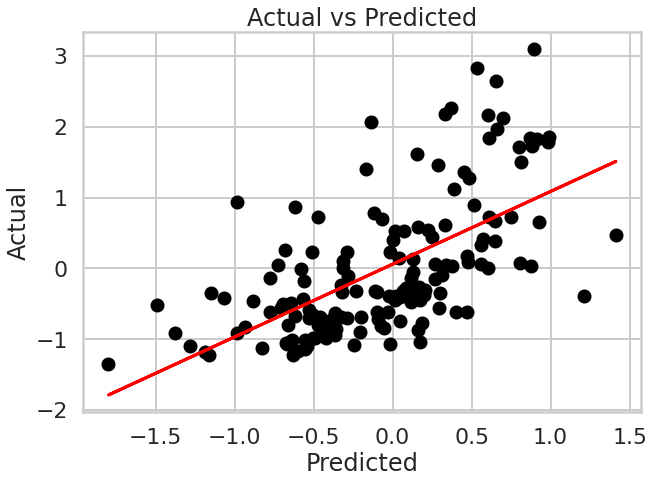
\includegraphics[width=0.6\linewidth]{figures/graphs/model_2_graph.png}
    \caption{Actual vs. Model 2 Predicted values }
  \label{fig:model2}
\end{figure}

% ----- Model 3
\subsection{Model 3: Feature Selection with Pearson Correlation}

\subsubsection{Model 3.1 Selected features (threshold=0.3)}

Table \ref{tab:model3_1} shows the intercept and coefficients of the model with selected features: watch time(minutes), stream time (minutes), partnered and mature.  \\

\begingroup
\setlength{\tabcolsep}{5pt} % Default value: 6pt
\renewcommand{\arraystretch}{1} % Default value: 1
\begin{table}[h]
    \centering
    \caption{Model 3.1 coefficients from linear regression with selected features: watch time (minutes), stream time (minutes), partnered, mature.}
    \begin{tabular}{|p{.10\linewidth}|p{.12\linewidth}|p{.20\linewidth}|p{.20\linewidth}|p{.15\linewidth}|p{.15\linewidth}|}
        \hline
      & \textbf{Int} & \textbf{Watch time (minutes)} & \textbf{Stream time (minutes)} & \textbf{Partnered} & \textbf{Mature} \\
     \hline
     \textbf{Coef} & 0.260330 & 0.762565	& -0.720557	& -0.273532	& 0.025943 \\
   \hline
    \end{tabular}
    \label{tab:model3_1}
\end{table}
\endgroup 

Figure \ref{fig:model3_1} shows the scatterplot of the actual 'average stream viewers' values against the predicted values of Model 3.1. It can be seen that the values are closely fitted to the regression line with the exception of some outliers, which indicates good performance from the model with correlation threshold=0.3. \\

\begin{figure}[h]
    \centering
    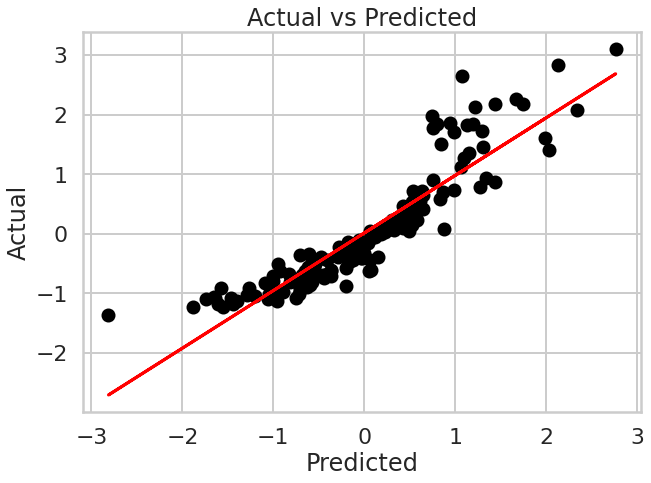
\includegraphics[width=0.6\linewidth]{figures/graphs/model_3_1_graph.png}
    \caption{Actual vs. Model 3.1 Predicted values }
  \label{fig:model3_1}
\end{figure}



\subsubsection{Model 3.2 Selected features (threshold=0.4)}

Table \ref{tab:model3_2} shows the intercept and coefficients of the model with selected features: watch time(minutes), stream time (minutes), peak viewers, partnered and mature. \\

\begingroup
\setlength{\tabcolsep}{5pt} % Default value: 6pt
\renewcommand{\arraystretch}{1} % Default value: 1
\begin{table}[h]
    \centering
    \caption{Model 3.2 coefficients from linear regression with selected features: Watch time(minutes), Stream time(minutes), Peak viewers, Followers, Partnered, Mature.}
    \begin{tabular}{|p{.08\linewidth}|p{.12\linewidth}|p{.15\linewidth}|p{.15\linewidth}|p{.10\linewidth}|p{.12\linewidth}|p{.14\linewidth}|p{.12\linewidth}|}
        \hline
      & \textbf{Int} & \textbf{Watch time (minutes)} & \textbf{Stream time (minutes)} &	\textbf{Peak viewers}	& \textbf{Followers}  & \textbf{Partnered} & \textbf{Mature} \\
     \hline
    \textbf{Coef} & 0.297777 &	0.72955 & 	-0.684541 & 0.064437 & 	0.028368 & 	-0.316929	& 0.043872 \\
   \hline
    \end{tabular}
    \label{tab:model3_2}
\end{table}
\endgroup 

Figure \ref{fig:model3_2} shows the scatterplot of the actual values against the predicted values of Model 3.2. The results are seen to have a few outliers and fit the regression line, suggesting that the model behaved well with a correlation threshold=0.4. \\

\begin{figure}[h]
    \centering
    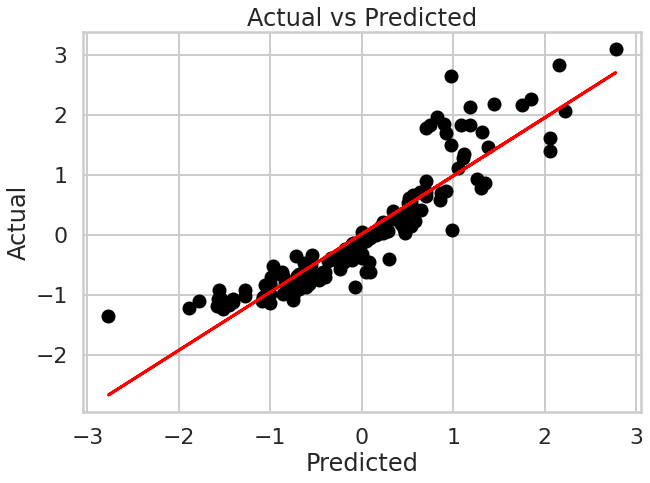
\includegraphics[width=0.6\linewidth]{figures/graphs/model_3_2_graph.png}
    \caption{Actual vs. Model 3.2 Predicted values }
  \label{fig:model3_2}
\end{figure}


\subsubsection{Model 3.3 Selected features (threshold=0.5)}

Table \ref{tab:model3_3} shows the intercept and coefficients of the model with all the features,  except views gained, with correlation threshold=0.5. \\

\begingroup
\setlength{\tabcolsep}{8pt} % Default value: 6pt
\renewcommand{\arraystretch}{1.2} % Default value: 1
\begin{table}[h]
    \centering
    \caption{Model 3.3 intercept and coefficients from linear regression with all the features,  except views gained.}
    \begin{tabular}{|p{.10\linewidth}|p{.14\linewidth}|p{.15\linewidth}|p{.15\linewidth}|p{.14\linewidth}|}
        \hline
      & \textbf{Int} & \textbf{Watch time (minutes)} & \textbf{Stream time (minutes)} &	\textbf{Peak viewers}\\
     \hline
     \textbf{Coef} &  0.295097 & 0.72971	& -0.680838	& 0.060772	\\
   \hline
    \end{tabular}
    \begin{tabular}{|p{.10\linewidth}|p{.14\linewidth}|p{.15\linewidth}|p{.15\linewidth}|p{.14\linewidth}|}
    \hline 
     & \textbf{Followers}	& \textbf{Followers gained} & \textbf{Partnered} & \textbf{Mature} \\
     \hline
    \textbf{Coef} & 0.021738	& 0.018391	& -0.314334	& 0.045911 \\
    \hline 
    \end{tabular}
    \label{tab:model3_3}
\end{table}
\endgroup

Figure \ref{fig:model3_3} shows the scatterplot of the actual values against the predicted values of Model 3.3. The results are also found to fit the regression line with a few outliers, showing that the model behaved well with a correlation threshold=0.5. \\

\begin{figure}[h]
    \centering
    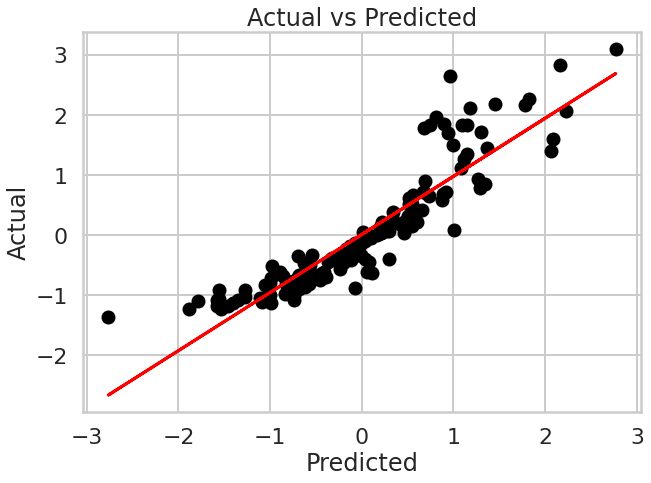
\includegraphics[width=0.6\linewidth]{figures/graphs/model_3_3_graph.png}
    \caption{Actual vs. Model 3.3 Predicted values }
  \label{fig:model3_3}
\end{figure}



\subsection{Evaluation of Models}

Table \ref{tab:eval} shows evaluation scores of all models for the following metrics: $ R^2 $, Mean Absolute Error (MAE), Mean Squared Error (MSE), Accuracy (Regression Score), and Cross-Validation Mean. \\

\begingroup
\setlength{\tabcolsep}{8pt} % Default value: 6pt
\renewcommand{\arraystretch}{1.2} % Default value: 1
\begin{table}[]
    \centering
    \caption{Summary of evaluation metrics scores of all models.}
    \begin{tabular}{|p{.15\linewidth}|c|c|c|c|c|}
        \hline
      \textbf{Model} & \textbf{ $ R^2 $} &	\textbf{MAE} & \textbf{MSE}	& \textbf{Accuracy} & \textbf{CV Mean}  \\
     \hline
     Model 1 & 0.805	& 0.287	& 0.163	& 0.827	& 70.890 \\
      \hline
     Model 2	& -0.713 &	0.602	& 0.586 & 0.379	&  -6.129 \\
      \hline
     Model 3.1	& 0.806 & 0.297	& 0.163 & 0.827 &	70.514 \\
    \hline
    Model 3.2 & 0.807	& 0.285	& 0.160  & 0.829	& 71.129 \\
    \hline 
    Model 3.3	& 0.805	& 0.287	& 0.163 & 0.827 & 71.051 \\
    \hline 
    \end{tabular}
    \label{tab:eval}
\end{table}
\endgroup 

All models, except Model 2, performed well in predicting the average viewers per stream in unseen data. Model 2 got the lowest $R^2$ (=-0.713) and accuracy (=0.379) scores, and the highest MAE and MSE scores. This rejects the hypothesis that the number of followers and total stream time (in a year) alone significantly affect the average viewers per stream of a Twitch streamer. \\

Meanwhile, Model 3.2 performed the best with the highest $R^2$ (=0.807) and accuracy (=0.829) scores, and the lowest MAE and MSE scores. This tells that the selected features with Pearson correlation namely, Watch time (minutes), Stream time (minutes), Peak viewers, Followers, Partnered, and Mature, contribute the most to the average viewers per stream of a Twitch streamer. \\

Thus, the best model for predicting the average viewers per stream or viewership for a Twitch stream is: 
\begin{equation}
    $
    \textbf{Average Viewers Per Stream} = 0.298 + 0.730 * \textit{Watch time (minutes)} - 0.685 * \textit{Stream time (minutes)} + 0.064  * \textit{Peak viewers} + 0.028 * \textit{Followers} - 0.317 * \textit{Partnered} + 0.044 \textit{Mature} 
    $
\end{equation}

\section{Conclusion}
The objective of this paper was to evaluate the factors that influence Twitch stream viewership. In doing so, three experimental setups were devised in order to understand the effects of the features against the average number of viewers. Setup 1 involved all of the features in the dataset, Setup 2 only involved the proposed features of higher viewership while Setup 3 involved feature selection using Pearson correlation and is subdivided into three thresholds=[0.3, 0.4, 0.5]. Linear regression was used to build models for each setup which were evaluated with the metrics: $ R^2 $, Mean Absolute Error (MAE), Mean Squared Error (MSE), Accuracy (Regression Score), and Cross-Validation Mean. \\

Except for Setup 2, all of the models scored well, with Model 3.2 showing the best evaluation results. The number of followers and total stream time in a year does not correlate with the average number of views per stream. However,  watch time, stream time, number of peak viewers, number of followers, and whether partnered and features mature content significantly contribute to or predict the average number of viewers per stream. These factors may be taken into consideration by aspiring and experienced Twitch streamers to maintain current viewership ratings or increase viewership in future streams.  \\ 

Further improvements of the models may be done by using a larger dataset, employing other feature selection methods, or by using other machine learning algorithms to build the models such as Huber regression. 


\newpage
% ---- Bibliography ----
\section{Bibliography}
\label{section-bibliography}
\bibliographystyle{IEEEtran}
\bibliography{twitch-viewership-factors}


\newpage
% ---- Appendix ----
\appendix
\section{Appendix}
\subsection{Dataset source}
The dataset used in this study is available online through Kaggle: \\
\texttt{https://www.kaggle.com/datasets/aayushmishra1512/twitchdata}

\subsection{Jupyter notebook}
Processes and computations done in this study can be viewed in this Jupyter notebook: \\
\texttt{https://github.com/yourstrulyhb/197-ML-mini-paper}



\end{document}
